%\newpage
\genHeader
\hypertarget{remCard end}{}
\subsubsection{Concluding removeCard}

Fantastic work! You have now implemented a simple method via patterns. As you can see, SDMs are effective for implementing structural changes in a high-level,
intuitive manner.

Let's take a step back and briefly review what we have specified:  if \texttt{p.remove\-Card(c)} is invoked for a partition \texttt{p}, with a card \texttt{c}
as its argument, the specified pattern will \emph{match} only if that card is contained in the partition. After determining matches for all variables, the
link between the partition and the card is deleted, effectively ``removing'' the card from the partition. If the card is \emph{not} contained in the partition,
the pattern won't match, and nothing will happen. In both cases, the card that's passed in is returned.

\begin{stepbystep}

\item If your code generation was successful, navigate to
``Learning\-Box\-Language/\-gen/\-Learning\-Box\-Language/\-impl/\-Partition\-Impl.java" to the \texttt{\-remove\-Card} declaration (approximately line 347).
Inspect the generated implementation for your method (\Cref{eclipse:remCardImpl}). Notice the null check that is automatically created - only a very
conscientious (and probably slightly paranoid) programmer would program so defensively!

\vspace{0.5cm}

\begin{figure}[htp]
\begin{center}
  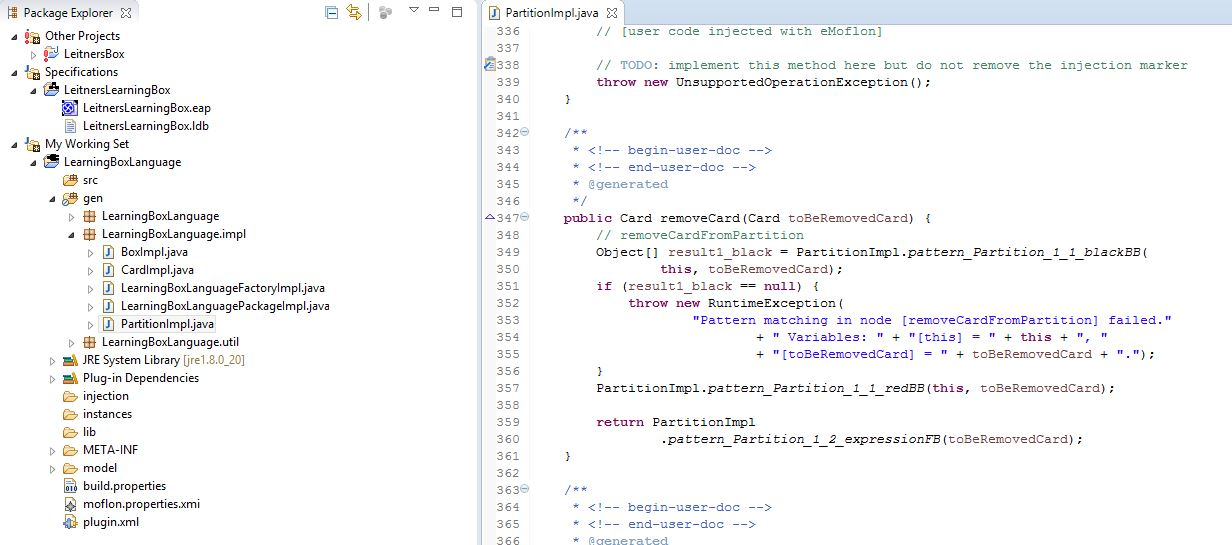
\includegraphics[width=\textwidth]{../../org.moflon.doc.handbook.03_storyDiagrams/03_removeCard/GUIImages/eclipse_remCardImpl}
  \caption{Generated implementation code}
  \label{eclipse:remCardImpl}
\end{center}
\end{figure}

\newpage

Near the end of Part II (after using injections), you were able to test this method's implementation using our \texttt{LeitnersBoxGui}. Let's run it again to
make sure \emph{this} version of \texttt{removeCard} works!

\item Load and run the GUI as an application,\footnote{Refer to Part II, Section 6 for details on our GUI} then go to any partition and
select \texttt{Remove Card} (\Cref{eclipse:GUIRemCard}).
It should immediately refresh, and you'll no longer be able to see the card in either the GUI or in the \texttt{Box.xmi} tree in the ``instances'' folder.
Pretty cool, eh?

\vspace{1cm}

\begin{figure}[htp]
\begin{center}
  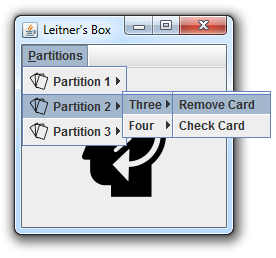
\includegraphics[width=0.5\textwidth]{../../org.moflon.doc.handbook.03_storyDiagrams/03_removeCard/GUIImages/eclipse_GUIRemove}
  \caption{Testing \texttt{removeCard}}
  \label{eclipse:GUIRemCard}
\end{center}
\end{figure}

\end{stepbystep}